\chapter{Methodology}
\label{ch:method}

\begin{figure}[!ht]
	\centering
	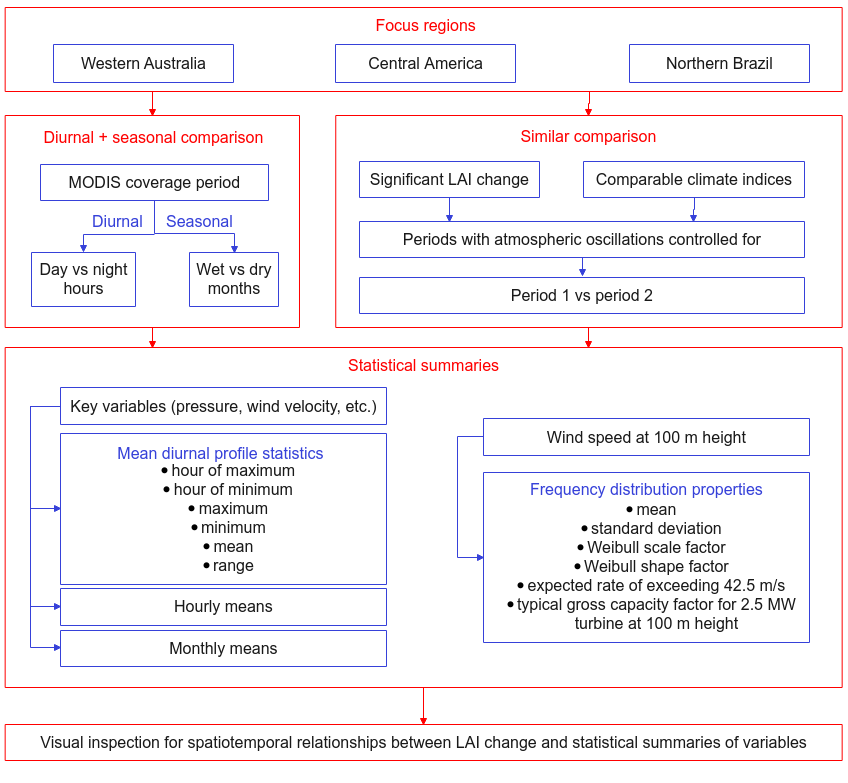
\includegraphics[width=0.9\textwidth]{method_flow.png}
	\caption[Methodology Flow Chart]{Flow chart summary for methodology. Results for all focus regions were obtained but only \acl{WA} was analysed due to project scope change (see Appendix~\ref{sec:other_regions}).}
	\label{fig:method_flow}
\end{figure}

\section{Approach}

\subsection{Spatiotemporal correlations}

To identify how vegetation loss may affect (or has historically affected) surface winds, we produced a series of spatial plots using \ac{GLASS} data \citep{liang2021} and \ac{ERA5} data \citep{era5}. These plots sought to uncover any spatiotemporal correlations between vegetation loss and key atmospheric variables such as wind speed, wind direction and mean sea level pressure. The rationale behind this was that were there to be any concrete spatiotemporal correlations, it would suggest strongly that there is some underlying dynamic between the variables (since a concrete pattern manifesting through both space and time purely by chance is unlikely), which may then shed some insight into how atmospheric circulations may change in the future.

In doing this, we first identified a focus region which was likely to yields meaningful results due to historically extensive degrees of vegetation change or other unique circumstances such as having a sharp delineation between natural and agricultural land cover. For this region, we produced three separate comparisons. 

\subsection{Diurnal comparison}

The first comparison was between the daytime and nighttime hours (which can have significant differences depending on land cover) for the period from Jan-2001 to Dec-2020\footnote{All period start and end dates in this report are inclusive unless otherwise stated.} (years in which available \ac{GLASS} data was most reliable due to an advancement of instruments), and will hereby be referred to as the "diurnal comparison".

\subsection{Seasonal comparison}

The second comparison was between the dry and wet seasons (which can have significant differences in vegetation). also for the period from Jan-2001 to Dec-2020, and will hereby be referred to as the "seasonal comparison".

\subsection{Similar comparison}

For the third and final comparison, we strategically selected two 5-year long historical periods with similar atmospheric conditions but extensive vegetation change, hereby referred to as the "similar comparison". Periods for the similar comparison were selected in such a fashion so as to control (to the extent possible) for other effects such as atmospheric oscillations which may also affect the key atmospheric variables of interest (mainly wind speeds, wind velocities and mean sea level pressure).

For each of these three comparisons, we then created a series of spatial plots displaying summary statistics for the key atmospheric variables (see Section~\ref{sec:method_var}), as well as differences in these statistics between seasons or periods (other related variables which might affect the behaviour of the key variables were also studied).

\subsubsection{Mean diurnal profile}

Central to these summary statistics was a variable's \ac{MDP} over each period, produced using a group-wise average by hour of day for all the data values in that period. This was computed for each grid cell in the data, and was used to study how vegetation change might affect the diurnal variations in key variables. Because of the difficulty in visualising the temporal variability in spatial data, we created plots for the hour of maximum, hour of minimum, maximum, minimum, mean and range of these \ac{MDP} values. We also created spatial plots for the mean values over each hour of the day and month of the year, to analyse cotemporaneous diurnal and seasonal evolution of different variables respectively.

\subsubsection{Wind speed distribution}

In addition to this, we created spatial plots for the wind speed distributional properties over each period (and the difference in these values between periods) for the wind speed at 100 m above surface such as its standard deviation, gross capacity factor for a typical wind turbine with 100 m hub height, empirical fits for the Weibull parameters, and the expected rate of exceeding 42.5 m/s (the typical speed which a turbine can withstand for 10 minutes).

\subsection{Visual inspection for trends}

Spatiotemporal correlations were then identified by visual inspection as this was deemed more appropriate than a rigid statistic metric, since the latter will have to be computed upon gridded data and hence may miss spatial correlations between variables which are present but manifest slightly offset from each other by a few grid cells (and it is a non-trivial task to systematically correct for all the different spatial variations by which two variables can be slightly offset from each other, if possible at all).

\section{Focus region}

\begin{figure}[!ht]
	\centering
	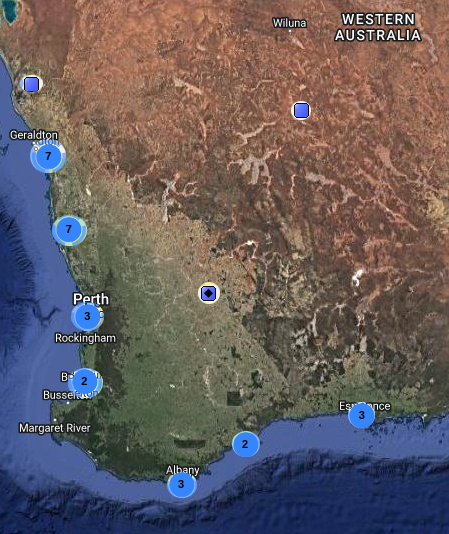
\includegraphics[width=0.75\textwidth]{maps_twp_wa}
	\caption[Western Australia Map]{Satellite image displaying Western Australia focus region from 114$^\circ$E to 124$^\circ$E longitude and 36$^\circ$S to 6$^\circ$S latitude \citep{maps_wa}. Markers indicating positions and number of wind farms have been edited on using data from \citep{twp_wa}. The State Boundary Fence of Western Australia sharply delineates agricultural vegetation on the west from native vegetation on the east.}
	\label{fig:maps_twp_wa}
\end{figure}

\subsection{Description of region}

We selected the south-west part of \ac{WA} (from 114$^\circ$E to 124$^\circ$E longitude and 36$^\circ$S to 6$^\circ$S latitude; see Figure~\ref{fig:maps_twp_wa}) for investigation because previous studies \citep{lyons1993, lyons1996, lyons2002, xinmei1995, ray2003, esau2002} have suggested significantly different atmospheric conditions on each side of the \ac{SBFWA}, which itself sharply delineates native vegetation (eastern side) from agricultural land (western side). The entire focus region is on the order of 1000 km, so synoptic weather features (which have a characteristic scale of this order) are less likely to produce contrasting effects over the different subregions.

Land surface characteristics on the agricultural side exhibit pronounced seasonal fluctuations due to the annual growing and harvest of wheat, after which the ground is left bare before the next growing season. This occurs along what is called the Wheat Belt Region of Western Australia (see Figure~\ref{fig:lc_wa}) where land usage has remained largely the same over recent decades. An excellent description of the terrain near Lake King (around the straight part of the fence) is provided by \citet{lyons2002}:

\begin{displayquote}
	The native vegetation is characteristically a woodland called mallee with \textit{Eucalyptus eremophila} the most consistent species. Patches of eucalypt woodland occur on lower ground and scrub heath and casuarina thickets are found on the residual plateau soil. The topography is gently undulating country of low relief with duplex mallee soils - that is, sand overlying clay. The native vegetation is between 0.5-6 m high, with more than 75\% of this vegetation between 0.5-2 m. The adjoining farmlands cultivate winter growing annual species. Wheat is the major crop in the agricultural area and grows between May and November. Crops are generally less than 1 m high during the growing season and after harvest stubbles of about 20 cm or bare soil are common.
\end{displayquote}

\begin{figure}[!ht]
	\centering
	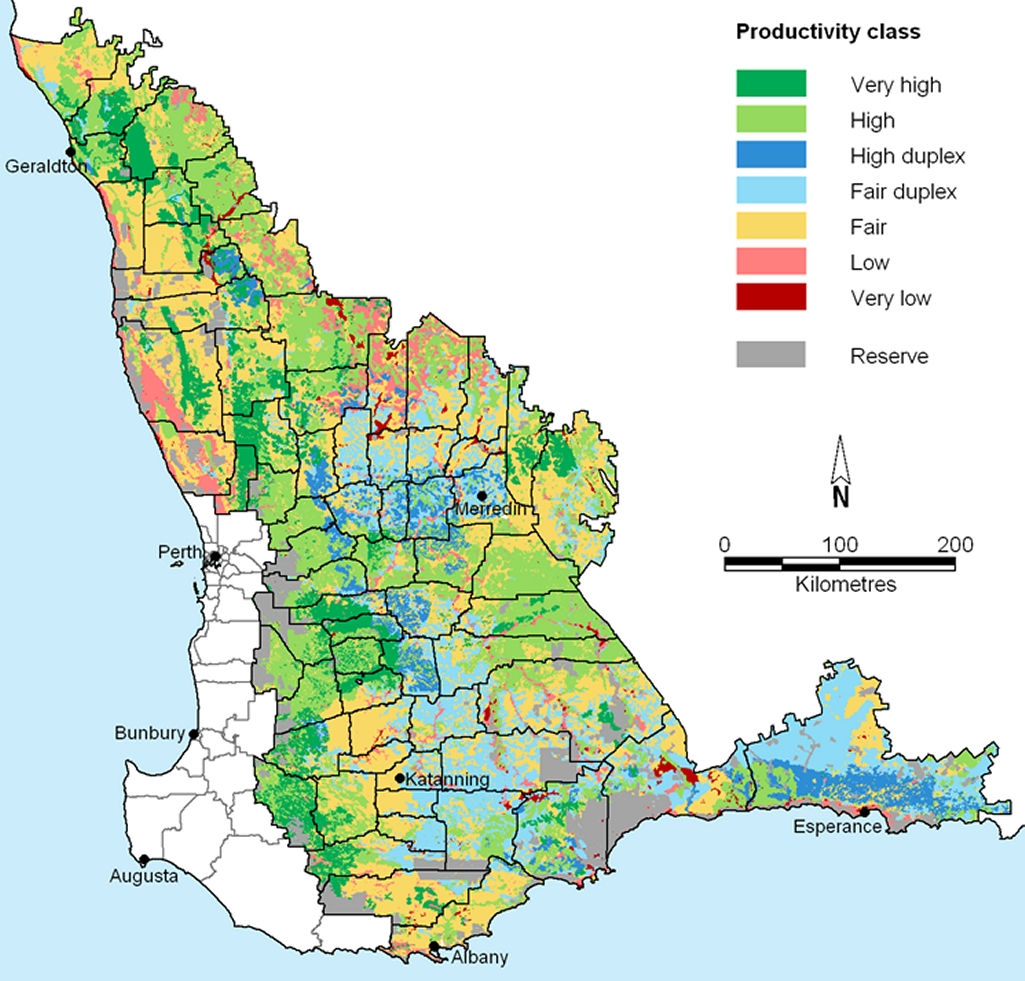
\includegraphics[width=0.75\textwidth]{lc_wa}
	\caption[Western Australia Land Usage]{The Wheat Belt of Western Australia, with shading indicating level of productivity \citep{lc_wa}.}
	\label{fig:lc_wa}
\end{figure}

\subsection{Significance of results from this region}

This focus region was selected mostly for these unique characteristics which are conducive towards eliciting insights into the general principles tying land cover with atmospheric circulation, but may also have some direct implications for wind farms in the area, most of which are situated along the coast (see Figure~\ref{fig:maps_twp_wa}). Vegetation change on an annual to decadal scale has been concentrated along the south-western coastal forests (see Figure~\ref{fig:wa_lai_similar}), while effects on a seasonal scale will be most pronounced along the fence. Wind farms around these subregions are the ones most likely to see a change in wind resource due to continued forest loss and future agricultural expansion respectively.

\section{Study periods for each comparison}

\subsection{Diurnal and seasonal comparisons}
\label{ssec:method_diurnal_seasonal}

The diurnal and seasonal comparison were performed over the period from Jan-2001 to Dec-2020 (inclusive). The GLASS products derived from \ac{MODIS}, the more advanced instrument, begin around Mar-2000, with the \ac{LAI} dataset ending Dec-2021 while the \ac{FAPAR} dataset ends Dec-2020 (at the time of writing). As averages starting from Mar-2000 and ending Dec-2020 would have skewed weightings for the months of January and February, we elected to use Jan-2001 as the period start instead.

The local timezone for \ac{WA} is UTC+8. Where comparisons between "daytime" and "nighttime" hours have been made, the average values for hours from 8 am to 3 pm \ac{LT}\footnote{Unless otherwise stated, all times in this report are expressed in local time, and hour endpoints are inclusive.} (8-9-10-11-12-13-14-15) have been selected as representative of daytime, while the average values for hours from 8 pm to 3 am local time (0-1-2-3-20-21-22-23) have been selected as representative of nighttime. Meanwhile, based on historical precipitation climatology, the months of \ac{JJA} and \ac{DJF} were selected as being representative of the wet and dry season respectively.

\subsection{Similar comparison}

To control for differences arising from atmospheric oscillations, and to select periods for which there was sufficient vegetation change for meaningful results to appear, we selected a set of study periods based on the following criteria (in order of priority):
\begin{enumerate}
	\item 5-year rolling averages for relevant climate indices were similar or at a similar phase in the oscillation
	\item Change in \ac{LAI} between the periods was extensive or had opposite trends in different subregions
	\item Monthly values for relevant climate indices over each period displayed a similar time evolution pattern
	\item Periods covered a similar amount of time spent in La Nina / El Nino events (where relevant) and Negative / Positive \ac{IOD} events (where relevant)
\end{enumerate}

Period lengths of 5 years were selected since this somewhat averages out the effect of shorter-term atmospheric fluctuations. To assist in the selection of periods, we created 5-year rolling average line plots for all major climate indices (see Section~\ref{ssec:indices}) but with a focus towards those corresponding to the focus region's relevant (i.e.\ climate-driving) atmospheric oscillations. We also created yearly spatial plots for the 5-year rolling average of the annual difference in \ac{MLAI} (see Section~\ref{ssec:mlai_diff}).

\subsubsection{Climate indices}
\label{ssec:indices}

5-year rolling average line plots were produced for the following climate indices using monthly data obtained from \ac{NOAA} \citep{ind_source}:
\begin{itemize}
	\item \ac{AMOI}, for the \ac{AMO}
	\item \ac{PDOI}, for the \ac{PDO}
	\item \ac{ONI}, for the \ac{ENSO}
	\item \ac{DMI}, for the \ac{IOD}
	\item \ac{AAOI}, for the \ac{AAO} / \ac{SAM}
	\item \ac{AOI}, for the \ac{AO} / \ac{NAM}
	\item \ac{NAOI}, for the \ac{NAO}
	\item \ac{EPOI}, for the \ac{EPO} / \ac{NPO}
\end{itemize}

Overlayed upon the \ac{ONI} graphs were windows indicating when La Nina and El Nino events have occurred in the past, as defined by the \ac{JMA}.\footnote{Note that different meteorological agencies define these events differently. \ac{JMA} definitions were used here because it was the only data down to a monthly resolution which was easily obtainable.} And overlayed upon the \ac{DMI} graphs were windows indicating when Negative \ac{IOD} and Positive \ac{IOD} events have occurred in the past, as defined by \ac{JMA}.

\subsubsection{Annual difference in mean leaf area index}
\label{ssec:mlai_diff}

For each calendar year with completed data in the \ac{GLASS} dataset, an annual mean value was computed for the \ac{LAI} at each grid point. The annual difference in \ac{MLAI} for each year was then defined as the \ac{MLAI} for that year minus the mean of the previous year. A 5-year rolling average centred upon each year was then produced by averaging the four annual differences calculated across the five annual means. For example, the 5-year rolling average for the year 2002 would be the average of $MLAI(2004)-MLAI(2003)$, $MLAI(2003)-MLAI(2002)$, $MLAI(2002)-MLAI(2001)$ and $MLAI(2001)-MLAI(2000)$, where the \ac{MLAI} over a given year is expressed as $MLAI(year)$.

This averages out the shorter term fluctuations which may be due to rainfall anomalies around a mean trend, or other factors such as changes in cropping. Although interesting in their own right, these are only indirectly related to \ac{LCC} (the subject of this report) and so are not pursued.

As the time difference between similar periods in terms of climate indices often exceeds 5 years, these plots were used only as a visual indicator to aid the selection process (to determine whether periods with sufficiently similar climate indices would also have extensive enough vegetation change to be worth studying). For final confirmation, separate comparison plots for the \ac{MLAI} over each of the selected 5-year periods were produced.

\section{Variables selected for analysis}
\label{sec:method_var}

\subsection{Main study variables}

The \acf{LSE} and \acf{SSGO} were static variables derived from the \ac{ERA5} dataset, used to identify whether orographically-induced circulations would be a confounding factor. \acf{MLAI} was the primary metric used to assess the extent of vegetation change, with \acf{MFAPAR} a secondary metric to corroborate results. 

We then selected out for analysis the \ac{ERA5} variables which were most relevant to our research goals. A full list of these variables is presented in Table~\ref{tab:vars_analysis} and also included are descriptions for wind speed distribution properties derived from \ac{ERA5} data (see Section~\ref{ssec:method_wsd}). But the main ones presented in the results are:
\begin{itemize}
	\item \acf{MSLP}
	\item \acf{WS100}
	\item \acf{dWS100}
	\item \acf{WV100}
	\item \acf{dWV100}
	\item \acf{T2}
	\item \acf{dT2}
	\item \acf{VIEC}
	\item \acf{NAC}
	\item \acf{VIDMF}
	\item \acf{NSE}
	\item \acf{VIKE}
	\item \acf{FA}
	\item \acf{SSHF}
	\item \acf{BLH}
\end{itemize}

\ac{MSLP}, \ac{WS100}, \ac{dWS100}, \ac{WV100} and \ac{dWV100} were natural inclusions given we are analysing the wind resource at heights relevant for wind energy generation. The other variables were targeted towards understanding the processes behind atmospheric circulation drivers, such as on surface energy balance, atmospheric energy conversions and possible effects of atmospheric condensation.

\subsection{Data fidelity}

There was an emphasis on variables related to water vapour transport, not only because of the potential for \ac{CIAD}, but also because this provides relatively high-fidelity data to corroborate the direction of tropospheric winds with that on the surface. Modelled outputs for water vapour transport are forced using satellite observations, and itself constitutes indirect measurement of tropospheric winds. But vegetation-surface wind interactions in ERA5 are modelled by extrapolating downwards from a fixed blending height and using grids with a characteristic roughness. As a result, the accumulated effects of sub-grid heterogeneity upon the trajectory of winds may not be accounted for, and in either case the surface winds are at least an extra step removed from direct measurement.\footnote{Observations assimilated into the model for \ac{ERA5} do not include wind velocity inputs from weather stations because \ac{ERA5} is averaged over 0.25$^\circ$ grids which makes it incompatible with \ac{WMO} conventions whereby 10 m winds are measured in open terrain. Instead, 100 m winds are extrapolated downwards from higher model levels under idealised assumptions, and the data assimilated for these higher model levels in turn derives from a mix of atmospheric soundings, aircraft and satellite irradiance data (part of which relies back on water vapour observations).}

\subsection{Net atmospheric condensation}

We also derived a variable called \ac{NAC}, which was meant to approximate the instantaneous balance between cloud formation and cloud evaporation at each hour of the day (see Appendix~\ref{sec:nac_derive} for derivation):
\begin{eqnarray}
	\label{eq:nac}
	NAC \ [kg m^{-2} s^{-1}] = NSE \ [kg m^{-2} s^{-1}] - VIDMF \ [kg m^{-2} s^{-1}] \\ 
	- \frac{d}{dt}(TCWV \ [kg m^{-2}]) \nonumber
\end{eqnarray}
where \acs{NSE} is the net evaporation at the surface (i.e.\ not including atmosphere), \acs{VIDMF} is the vertical integral of divergence of moisture flux, and \acs{TCWV} is the total column water vapour (see descriptions in Table~\ref{tab:vars_analysis}).

\subsubsection{Atmospheric water budget equation}

This is an accounting equation arising from the fact that \ac{TCWV} can only change either due to net evaporation or condensation (on the surface and also in the atmosphere), or movement of water vapour from a neighbouring column (it is also theoretically possible for chemical reactions and sublimation/deposition to add or remove water vapour but this is assumed negligible). This equation is usually expressed in the atmospheric water vapour budget literature \citep{norris2020, yan2020} as
\begin{eqnarray}
	\frac{d}{dt}(TCWV) = E - P - VIDMF
\end{eqnarray}
where E is surface evaporation and P is precipitation. But this equation is only valid for larger spatial and temporal scales. 

At larger temporal scales, surface evaporation at the surface typically exceeds surface condensation, so \ac{NSE} will be positive and is expressed as E (but note that this is using a more abstract notion of “surface evaporation” which absorbs the effect of intermittent surface condensation within the study period). To avoid confusion, we retain the use of the term “NSE” which makes explicit that surface condensation is absorbed within this variable. 

Also, this literature equation is only valid if P = NAC. All atmospheric condensation eventually falls as precipitation so this equation is valid on larger spatial and temporal scales. But on smaller scales, there may be several hours of delay between condensation and precipitation, and winds may blow the condensed water droplets across several hundred km before precipitating. Since we are studying hourly diurnal profiles and using 30 km grids, we opt for \ac{NAC} rather than P in this equation.

By similar reasoning, the use of \ac{TCCLW} may give misleading results since prevailing winds may low cloud liquid water far from their point of formation. Thus, \ac{NAC} is meant to provide a more accurate depiction of where cloud formation is occurring.

\newpage

\section{Statistical summaries}
\label{sec:method_stats}

\begin{figure}[!ht]
	\centering
	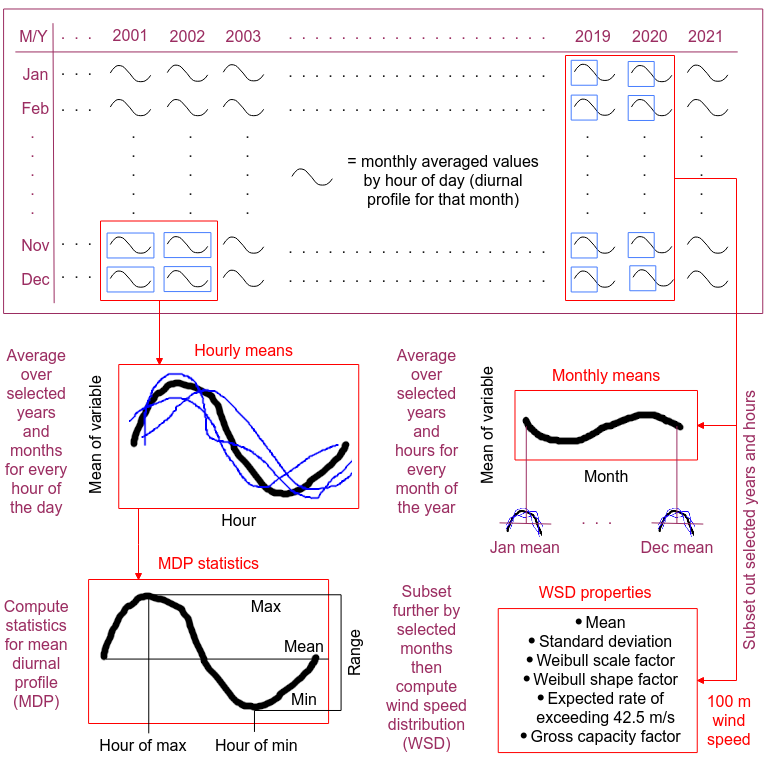
\includegraphics[width=0.9\textwidth]{stats_flow}
	\caption[Statistics Flow Chart]{Flow chart illustrating how the statistical summaries for each variable were computed.}
	\label{fig:stats_flow}
\end{figure}

\subsection{Mean diurnal profile statistics}
\label{ssec:method_mdp}

The "mean diurnal profile" (\ac{MDP}) for a variable was defined by computing groupwise means for values by hour of day\footnote{These averages were produced mostly by computing the mean of monthly averaged by hour of day data, which is roughly equivalent to the mean of all hourly data values. Vector variables were computed using hourly data values rather than monthly averaged by hour of day. Reasons for these choices are discussed in Appendix~\ref{sec:commutativity}.}. That is, the mean over all data values occurring on the first hour of the day were computed, then the same was done for the second and all subsequent hours up until the 24th hour, and together these constitute the \ac{MDP}. The \ac{MDP} can be computed upon a month subset of the total data available over a period, so \ac{MDP}s using values only from the wet or dry season can be obtained. 

The hour of maximum, hour of minimum, maximum, minimum, mean and range for the \ac{MDP} at each grid cell was then computed for visualisation\footnote{Note here that for variables which can take on both positive and negative values, maximum refers to the most positive \ac{MDP} value and minimum refers to the most negative \ac{MDP} value.}. Because, hour of maximum, hour of minimum, maximum, minimum and range for a vector is not well defined, we choose to apply generalised definitions for these statistics here so that: \ac{MDP} hour of maximum and minimum refers to when the \ac{MDP} magnitude of vector $\vec{v}$ is at a maximum and minimum respectively, \ac{MDP} maximum and minimum refers to the \ac{MDP} vector quantity of $\vec{v}$ at the hour of maximum and minimum, and \ac{MDP} range refers to largest magnitude of all possible subtractions (corresponding to all possible hourly combinations) between the 24 \ac{MDP} $\vec{v}$ values. Formally:
\begin{eqnarray}
	hour_{max}(\vec{v}) = i \mbox{ where } |\vec{v}_i| = max( \{|\vec{v}_k| : k \in \mathbb{Z} \cap [1,24] \}) \\
	hour_{min}(\vec{v}) = j \mbox{ where } |\vec{v}_j| = min( \{|\vec{v}_k| : k \in \mathbb{Z} \cap [1,24] \}) \\
	max(\vec{v}) = \vec{v}_i \mbox{ where } |\vec{v}_i| = max( \{|\vec{v}_k| : k \in \mathbb{Z} \cap [1,24] \}) \\
	min(\vec{v}) = \vec{v}_j \mbox{ where } |\vec{v}_j| = min( \{|\vec{v}_k| : k \in \mathbb{Z} \cap [1,24] \}) \\
	mean(\vec{v}) = \frac{1}{24} \sum_{k=1}^{24} \vec{v}_k \\
	range(\vec{v}) = max(\{|\vec{v}_k - \vec{v}_l| : k,l \in \mathbb{Z} \cap [1,24] \})
\end{eqnarray}

\subsection{Hourly means}

Hourly mean values are equivalent to the actual hourly values which constitute the \ac{MDP} (as opposed to the \ac{MDP} statistics).

\subsection{Monthly means}

Monthly mean values are similar to hourly means except that it is computed separately for every month of the year (rather than a collection of months corresponding to wet or dry season), and instead can be computed over a subset of hours for comparison between day and night hours.

\subsection{100 m wind speed distribution}
\label{ssec:method_wsd}

\subsubsection{Empirical Weibull fit}

For the wind speed distribution, the sample mean and standard deviation was first obtained over the selected months and hours subset. An empirical Weibull fit was then performed in accordance with the methodology outlined by \citep{justus1977}:
\begin{eqnarray}
	k = \left( \frac{\sigma}{\bar{V}} \right)^{-1.086} \\ 
	c = \frac{\bar{V}}{\Gamma (1 + 1/k)}
\end{eqnarray}
where $k$ is the Weibull shape parameter, $c$ is the Weibull scale parameter, $\sigma$ is the standard deviation of wind speed, $\bar{V}$ is the mean of wind speed, and $\Gamma (z) = \int_0^\infty t^{z-1} e^{-t} dt$ is the gamma function.

\subsubsection{Expected rate of exceedance}

\ac{EROE100} was then calculated using the tail from the empirical Weibull fit (as opposed to rate of exceedance directly calculated from the hourly data points) since the underlying probability distribution better captures risks which by chance may not have manifested in the data points. 42.5 m/s was chosen as this is the typical wind speed which wind turbines can last 10 mins in before failure \citep{chen2015, chen2016, ge_web}.

Experimental results by \citet{lee2012} and a review of methods by \citet{palutikof1999} suggest that the use of a Gumbel distribution for wind gust data would have been more accurate for assessing extreme wind speeds, but this analysis was not pursued since the ERA5 dataset does not contain a field for wind gusts at 100 m, and because interpretation of Gumbel parameters are less intuitive.

\subsubsection{Typical gross capacity factor at 100 m}

As opposed to EROE100, \ac{TGCF100} was directly calculated from the hourly data points. This was deemed valid because tail wind speeds have an insignificant effect on \ac{TGCF100} as all wind speeds above the cutoff represent zero power anyway. \ac{TGCF100} was calculated by first averaging the power curves of three turbines by common manufacturers to obtain a typical power curve, then using this to calculate the average power generated over the period as a fraction of the nameplate power rating.\footnote{Note that this is mathematically equivalent to computing the gross capacity factor for each of the three turbines then finding the average (see Appendix~\ref{sec:commutativity}).} The Vestas V100/2600, Goldwind GW100/2500 and GE Energy 2.5-100 were chosen for this calculation since these were turbines at 100 m hub height with comparable rotor diameter (100 m), power rating (2500 kW), and cut-in and cut-off wind speeds.\footnote{The Vestas power curve was scaled by a factor of 25/26 to make it comparable with the other turbines.} Data for these turbine power curves were obtained from \citet{twp_ge, twp_gw, twp_vt}.

\section{Main datasets}

\subsection{ERA5 reanalysis data}

The \ac{ERA5} dataset is provided by \ac{ECMWF} and is widely used in atmospheric studies and is considered one of the more accurate reanalysis datasets for surface wind speeds \citep{era5, torralba2017, ramon2019, clarke2021, fan2021}. We required reanalysis data to visualise spatially complete changes over an entire region (as opposed to in-situ measurements which are usually sparse). Of the available reanalysis datasets, ERA5 was chosen for its superior spatial (0.25$^\circ$) and temporal (hourly) resolution, closest agreement with observed wind speeds, and relatively accurate capture of interannual variability \citep{torralba2017, ramon2019, clarke2021, fan2021}.

The superior resolution was particularly important since this project sought to investigate diurnal variations (so an hourly time resolution was desirable), and the methodology was designed to interrogate the interfaces between different types of land cover (coarser spatial resolutions may have averaged out interesting effects).

\subsection{GLASS satellite-derived data}

The \ac{GLASS} product suite includes spatially complete modelled datasets for \ac{LAI} and \ac{FAPAR} with temporal resolution of 8 days (constrained by satellite overpasses) and spatial resolutions down to 250 m. This dataset is widely used for analysing vegetation cover and land surface effects \citep{fang2019, liang2021}, and was selected because it was found to be the most consistent with Google Earth historical satellite imagery. The datasets with spatial resolution of 0.05$^\circ$ were selected as this provided sufficient detail to distinguish land cover types at sharp interfaces without consuming too much computer storage and memory.

Other datasets such as the \ac{ERA5} \ac{LAI} variables \citep{era5}, \ac{C3S} \ac{LAI} V3 \citep{c3s}, \ac{NOAA} \ac{CDR} \ac{LAI} V5 \citep{lai_noaa} and \ac{NOAA} \ac{CDR} \ac{NDVI} V5 \citep{ndvi_noaa} were considered, but these were found to often have missing values, data processing artefacts, discrepancy against Google Earth historical satellite imagery, or other significant data deficiencies (not shown).

\section{Software}

All data manipulations were performed using Python 3.9.12. Statistical summaries were computed primarily using the \verb+xarray+ \citep{xarray} and \verb+dask+ \citep{dask} libraries, while visualisations relied on the \verb+matplotlib+ \citep{matplotlib} and \verb+cartopy+ \citep{cartopy} libraries.

A series of purpose-designed Python programs were created in the course of this project. These programs include a \verb+data_download.py+ script to automatically download all raw data inputs used in this project, a \verb+calc_funcs.py+ script which handles all the data processing, and a \verb+plot_funcs.py+ script which handles all the visualisations. 

All programs created in the course of this project are freely available, and all results were designed to be reproducible from scratch (see Appendix~\ref{app:code}). With trivial edits, these programs can take an arbitrary variable from the ERA5 dataset, then compute and visualise the statistical summaries outlined in Section~\ref{sec:method_stats}. These programs have broader applicability beyond this project as it can be used to study diurnal and seasonal variations in general, as well as how these variations differ between periods.

Due to the memory requirements necessary to process the large datasets, this research includes computations using the computational cluster Katana supported by Research Technology Services at \ac{UNSW} Sydney.